\documentclass[sigconf,natbib=false,10pt]{acmart}

%% Rights management information.  This information is sent to you
%% when you complete the rights form.  These commands have SAMPLE
%% values in them; it is your responsibility as an author to replace
%% the commands and values with those provided to you when you
%% complete the rights form.


\setcopyright{rightsretained}
\copyrightyear{2021}
\acmYear{2021}
\setcopyright{rightsretained}
\acmConference[HotOS '21]{Workshop on Hot Topics in Operating Systems}{May 31-June 2, 2021}{Ann Arbor, MI, USA}
\acmBooktitle{Workshop on Hot Topics in Operating Systems (HotOS '21), May 31-June 2, 2021, Ann Arbor, MI, USA}
\acmDOI{10.1145/3458336.3465284}
\acmISBN{978-1-4503-8438-4/21/05}
\hyphenation{pseu-do-ny-mi-za-tion pseu-do-ny-mizes sche-mas}


% to be able to draw some self-contained figs
\usepackage{tikz}
\usepackage{amsmath}
\usepackage{hyperref}
\usepackage[normalem]{ulem}
\usepackage{listings, listings-rust}
\usepackage{xspace}
\usepackage{booktabs}
\usepackage{multirow}
\usepackage{wasysym}
\usepackage{caption}
\usepackage{subcaption}
\usepackage{enumitem}
\usepackage[utf8]{inputenc}
\usepackage[compact, small]{titlesec}

\captionsetup{labelfont=bf,textfont=rm,belowskip=-8pt,aboveskip=8pt}

% BibLaTeX for bibliography
\usepackage[
  backend=biber,
  style=numeric-comp,
  minalphanames=3,
  isbn=false,
  sortcites=true,
  sorting=anyt,
  abbreviate=false,
  url=false,
  doi=false,
  maxnames=99,
  minbibnames=3,
  maxbibnames=99]{biblatex}
\addbibresource{paper.bib}

%\newcommand{\sys}{Couturier\xspace}
%\newcommand{\sys}{Fashionista\xspace}%Sidekick
\newcommand{\sys}{Edna\xspace}
\newcommand{\lrtbf}{\texttt{Lobsters-GDPR}\xspace}
\newcommand{\hrtbf}{\texttt{HotCRP-GDPR}\xspace}
\newcommand{\hrtbfplus}{\texttt{HotCRP-GDPR+}\xspace}
\newcommand{\hconfanon}{\texttt{HotCRP-ConfAnon}\xspace}

\newcommand{\gdpr}{\texttt{GDPR}\xspace}
\newcommand{\ca}{\texttt{ConfAnon}\xspace}

\newcommand{\thing}{guise\xspace}
\newcommand{\things}{guises\xspace}
\newcommand{\Things}{Guise\xspace}
\newcommand{\Thing}{Guises\xspace}

\newcommand\ms[1]{\textcolor{red!55!blue}{[malte: {#1}]}}
\newcommand\lyt[1]{\textcolor{green!55!blue}{[lyt: {#1}]}}
\newcommand\eddie[1]{\textcolor{blue!55!blue}{[E: {#1}]}}
\newcommand{\tabitem}{~~\llap{\textbullet}~~}
\newcommand{\eg}{{e.g.},\xspace}
\newcommand{\ie}{{i.e.},\xspace}


\definecolor{codegreen}{rgb}{0,0.4,0}
\definecolor{codegray}{rgb}{0.5,0.5,0.5}
\definecolor{codepurple}{rgb}{0.58,0,0.82}
\definecolor{backcolour}{rgb}{0.95,0.95,0.92}

\lstdefinestyle{rust}{
    %backgroundcolor=\color{backcolour},
    commentstyle=\color{codegreen},
    keywordstyle=\color{codepurple},
    stringstyle=\color{blue},
    basicstyle=\ttfamily\scriptsize,
    breakatwhitespace=false,
    breaklines=true,
    captionpos=b,
    keepspaces=true,
    showspaces=false,
    showstringspaces=false,
    showtabs=false,
    tabsize=2
}
\lstset{style=rust}

%-------------------------------------------------------------------------------
\begin{document}
%-------------------------------------------------------------------------------

%don't want date printed
\date{}

%%
%% The "title" command has an optional parameter,
%% allowing the author to define a "short title" to be used in page headers.
% make title bold and 14 pt font (Latex default is non-bold, 16 pt)
\title{Privacy Heroes Need Data Disguises}
%\name-ing Your Data from the Internet }
%An Invisibility Cloak for the Internet}

%%
%% The "author" command and its associated commands are used to define
%% the authors and their affiliations.
%% Of note is the shared affiliation of the first two authors, and the
%% "authornote" and "authornotemark" commands
%% used to denote shared contribution to the research.
\author{Lillian Tsai}
\affiliation{%
  \institution{MIT CSAIL}
%\email{tslilyai@mit.edu}
%\affiliation{%
%  \institution{MIT}
%  \state{}
  \country{}
}
\author{Malte Schwarzkopf}
\affiliation{%
  \institution{Brown University}
%\email{malte@cs.brown.edu}
%\affiliation{%
%  \institution{Brown University}
%  \state{RI}
  \country{}
}
\author{Eddie Kohler}
\affiliation{%
  \institution{Harvard University}
%\email{kohler@seas.harvard.edu}
%\affiliation{%
%  \institution{Harvard University}
%  \state{MA}
  \country{}
}

\begin{abstract}
    Web applications face increasing legal and user demands to properly protect and manage user
    data, whether through supporting user's right to be forgotten, removing unnecessary or old user
    data, or moderating user content.
    %
    Meeting these demands to \emph{mask} data requires that applications perform the appropriate
    data transformations to sufficiently de-identify or modify data, while still retaining the data
    required for application utility or legal purposes. Because such transformations are necessarily
    application-specific and require handling complex data correlations, today's applications often
    forgo these transformations, or use ad-hoc methods with unclear guarantees to achieve them.
    %

    To help developers flexibly support data masking transformations in new and existing
    applications, we design and implement \sys, a system that takes as input a high-level
    specification of a transformation, and automatically applies it to the application database.
    \sys relies on the key abstractions of application \emph{entity graphs} and \emph{ghost
    entities}, which allow developers to express and automate practical transformations without
    onerous labor.
\end{abstract}

\iffalse
%
\name is a new data ownership paradigm for web services in which users subscribe to
services by granting a \emph{lease} of their data, instead of having a permanent account.
%
When the lease ends, the user switches from an identity-revealing
subscribed mode into a privacy-preserving unsubscribed mode, where the
service only retains anonymized data about them.
%
This paradigm strikes a balance between current practices that give services control over user
    data with low user privacy; and the opposite extreme that decouples user data from
    services for strong privacy, but breaks current business models and reduces service utility.
%achieves better user privacy and data protection than today's services, 
%but without making impractical assumptions or breaking current business models.
%
Under \name, users withdraw from a service without permanently losing access,
as they can resubscribe at any time, and one user's withdrawal does not affect
the service's utility for others.

%
A prototype design and implementation for \name suggests it can be realized
efficiently and with low burden for application developers.
%
%\ms{We should give our paradigm a name!}

%The paper proposes a new web application \emph{subscription paradigm},  Users flexibly switch between a privacy-preserving unsubscribed mode and an
%identity-revealing subscribed mode at any time without permanently losing their data. 
%This subscription paradigm strikes a balance between applications having complete ownership of user
%data, and completely decoupling user data from applications at the cost of application utility. 
%To solve the complex data retention and de-identification challenges associated with subscription,
%we design \name{}, a practical system that provides abstractions and mechanisms to help
%developers of databased-backed web applications achieve correct, privacy-compliant user
%unsubscription and resubscription without onerous labor.
\fi


\maketitle
%\vspace{-2\baselineskip}

%\lyt{NOTE: need to add page numbers somehow, fix formatting, add info to authors?}

%-------------------------------------------------------------------------------
\section{Introduction}
%-------------------------------------------------------------------------------

Web application users are more aware of their data privacy rights than ever before. 
Laws such as the European Union's General Data Protection Regulation (GDPR)~\cite{eu:gdpr} and
California's Consumer Privacy Act (CCPA)~\cite{ca:privacy-act} codify users' rights to 
data ownership, granting users the right to request erasure of information related to them.
%
Public news around web services increasingly emphasize the dangers of leaving private data on the
web: embarrassing or compromising details from the past has reemerged, web applications have 
suffered data leaks or hacks, and private data has be shared by web applications without the user's
knowledge or explicit consent~\cite{nytimes:fb, npr:data}.

%
For the first time, companies face both legal and societal demand to support \emph{unsubscription}
of users from their services. Users have the right to unsubscribe at any time, preventing 
idle or unused accounts from retaining personal data indefinitely, and regaining control over who
can access their data. 
%

%
Unsubscription, however, is only half the story. Users cannot truly regain their data rights if they
are impeded from exercising them.  In order to claim that users have regained ownership of their
data, users must be freely able to exercise their right to be forgotten. In particular, they should
not have to pay a high price in order in order to unsubscribe whenever they wish: web services
should not raise barriers to unsubscription that prevent users from choosing to do so, when they
would have otherwise. These barriers can take several forms, from UI choices that hide paths to
unsubscription, to the threat of permanent deletion of years or even decades of accumulated
application data.

To empower users to freely exercise their data rights, web applications must allow users to easily
unsubscribe \emph{and resubscribe} as they wish, switching between a privacy-preserving unsubscribed
mode and an identity-revealing subscribed mode at any time without permanently losing their data, or
needing to maintain their account data themselves. 
%
With this model of flexible privacy, the balance of data ownership flips. Applications no longer
control users' data choices by demanding that users choose between indefinitely giving up their data
to use the application, or permanently losing their data and application utility.
Instead, users lease out their data for limited periods of time in exchange for the ability to use the application for 
that period, and lose no application utility between leases.
%\lyt{Users could do this without
%application support by themselves by programmatically setting a personal reminder to ``unsubscribe
%after x days'' every time they create an account.}
%

In the rest of this paper, we describe the current unsubscription and resubscription support (and
lack of support) in today's web applications, and the challenges of doing so correctly.
We then describe \sys, a system that provides abstractions and mechanisms
that help developers of databased-backed web applications achieve correct,
privacy-compliant user unsubscription and resubscription without onerous labor, and without adding
undue overheads.

\section{Challenges of Privacy Transformations}
\label{sec:motivation}
%
%We investigate the potential of privacy transformations as a first-class
%citizen in application design, and the challenges to support these
%transformations.
%%
%These challenges argue for a systematic approach to privacy transformations.
%%

%
Implementing privacy transformations combines two key challenges: the broad
range of possible policy choices for transformations, and the difficulty of
implementing those policies.
%
The first challenge can be appreciated by surveying current applications.
%
For example, though many applications support account deletion,
some retain
data for legal or necessary business purposes (\eg Spotify fraud detection~\cite{spotify:privacy},
Amazon orders~\cite{amazon:privacy}); some delete public contributions, but keep private
messages unanonymized and visible to their recipients, reflecting the
shared nature of such messages~\cite{facebook:privacy, twitter:privacy};
and yet others keep public contributions visible but anonymize them, reattributing the contribution
to a placeholder user (\eg GitHub's ``@ghost''~\cite{github:privacy}, Reddit/Lobsters'
``[deleted]''~\cite{reddit:privacy, lobsters:privacy}).
%
A system aiming to simplify privacy transformations must thus support a range
of operations, and implement application-defined policy.


The second challenge arises because privacy transformations are
inherently difficult (they require extensive tracing of user identities through
application data schemas), but also secondary to normal application
functionality.
%
Modifying or deleting data must not compromise application correctness; for example, privacy
transformations must maintain referential integrity of an application's relational database
and preserve other application invariants.
%
Furthermore, one application may apply support several interacting privacy
transformations.


The complexity of implementing basic transformations may have discouraged
developers from supporting more nuanced transformations.
%
This is too bad, because where privacy is concerned, nuance could benefit 
users.
%
For example, here are some useful policies that few applications currently
support.

\begin{itemize}
\item GDPR and related laws focus on irrevocable account deletion, where
a user departing a platform causes permanent deletion of their information.
However, users may be more likely to proactively protect their privacy if they
can return: if the deletion transformation is \textbf{reversible}.
%
A weak form of reversible transformation might preserve user data in the
application's normal database; though this hides the data from external view,
it leaves it at risk to breaches and does not satisfy most legal requirements.
Stronger forms are possible, however. The records required to reverse a
transformation might be stored offline, in other data storage layers, or even
encrypted and passed to the user themselves.

%Furthermore, many applications might wish to employ \textbf{reversible}
%transformations to, for example, support account reactivation instead of
%permanent and irrevocable account deletion.

\item \textbf{Expiration} policies could proactively anonymize or sanitize
user contributions for long-inactive users. Expiration policies should likely
be reversible to support user reactivation.

\item Gradual \textbf{data decay} policies could apply increasingly strict privacy transformations
    over time, aging out sensitive but outdated user contributions.
%for increasingly sensitive users, or gradually, over time.
\end{itemize}
%
These policies, and especially reversible transformations, were central to our
thinking as we developed the data disguise paradigm.



\begin{comment}

\eddie{END SECTION HERE?}

%
%
%Finally, practical privacy transformations should require minimal application changes.
%

%
To make these challenges concrete, consider implementing two privacy
transformations in HotCRP~\cite{hotcrp}:
%
(1) \gdpr implements GDPR's ``right-to-be-forgotten'' removal of user
data; and
%
(2) \ca anonymizes reviewers in the database some time after the
reviewing concludes, preventing reviewer identification in case of a data breach.
%
\ca needs to decorrelate reviews and review metadata (\eg review preferences)
from reviewers by ensuring that nothing associated with a review references a real user's
account by foreign key.
%
To maintain referential integrity, the developer must take care to generate fake user profiles
and update foreign key attributes to reference them.
%
The \gdpr transformation, by constrast, must identify all data related to a user and
remove it.%, though taking care to leave behind shared data such as review text.
%

%
In isolation, each transformation may seem simple; however, composing them is tricky.
%
\ca destroys information that links a user's data to their account by changing
that data to reference anonymous, fake users (\eg rewriting the foreign key for a review's
author to point to a fake user profile).
%
If this reviewer user later invokes \gdpr, the transformation needs to know which
data to remove, which is impossible without the original foreign keys.
%
%Due to data dependencies between these transformations, \texttt{GDPR} fails to achieve its desired
%privacy properties, namely the complete removal of the user's data.
%
When applied the other way around (\gdpr, then \ca) the transformations
compose more easily, as there is no need to anonymize deleted data.
%
But it falls to the application developer to write privacy transformation code that handles
both sequences of disguises correctly.
%

%\subsection{Utility of Privacy Transformations}
%If we can address these challenges, privacy transformations have the potential to provide many
%privacy benefits to web applications and their users.
%Widely-used web applications today~\cite{spotify:privacy, amazon:privacy,
%strava:privacy, hotcrp:privacy, wikipedia:privacy, facebook:privacy, twitter:privacy,
%reddit:privacy, github:privacy, lobsters:privacy} mainly support variants of an account
%deletion privacy transformation, as requried by, \eg the GDPR~\cite[Art.\ 17]{eu:gdpr}.
%
These challenges only become more urgent if we consider other desirable privacy transformations.
%
%But many applications would benefit from support for other privacy transformations.
%
%Users and application developers can both benefit from \textbf{more nuanced} privacy policies:
%for example, a confidential paper review system like HotCRP~\cite{hotcrp} keeps users'
%contributions (papers, reviews) after they delete their account to preserve utility for others, but
%could additionally associate each review with a different placeholder to avoid revealing the deleted
%reviewer's identity.
%
%Likewise, contributions with a shared property (\eg Reddit posts with a common tag)
%might be removed entirely to avoid inference attacks, or retained and decorrelated from the
%property (\ie keeping the user's Reddit posts, but removing their tags).
%\eddie{Would like more explanation of that}
%In some cases, a policy could preserve utility while reducing the efficacy of later inference
%attacks by \eg modifying sensitive metadata (\eg tags, creation times).
%
%Some transformations should be performed only on sensitive metadata:
%Similar policies could apply \emph{only if} the property was created by the user (\eg keeping
%the user's Reddit posts, but removing any user-created tags),
% tag like “\#cat” is likely insensitive and useful to preserve, whereas one naming a person is not.
%
%(\eg remove the user's posts on Reddit with tag $t$ if these posts comprise more than 10\%
%of all posts with tag $t$).
%
%Individual users could even specify different preferences for their data.
%
%% A privacy transformation framework is necessary to turn these preferences into concrete
%% operations without undue developer burden.
%
%
Applications could go beyond simple account deletion and support \textbf{data
expiration} policies, which anonymize a user's contributions after the user has been inactive for a
period of time, possibly restoring the user's profile and contributions if the user ever logs back
in.
%
Or the application could support gradual \textbf{data decay} policies that ``decay'' sensitive data
by applying incremental privacy transformations over time.

Furthermore, many applications might wish to employ \textbf{reversible} transformations to, for
example, support account reactivation instead of permanent and irrevocable account deletion.
%
After all, if services must allow users to remove their data on request, it is in the operator's
interest as well as the user's to make it easy for a user to change their mind and return, bringing
their data along.

We envision that a systematic approach to privacy transformations can help address the challenges
identified; if we can overcome these challenges, privacy transformations have the potential to enhance application
privacy beyond what we have discussed here.

\end{comment}

%-------------------------------------------------------------------------------
\section{Data Disguising}
%-------------------------------------------------------------------------------
\begin{figure}[t]
    \centering
    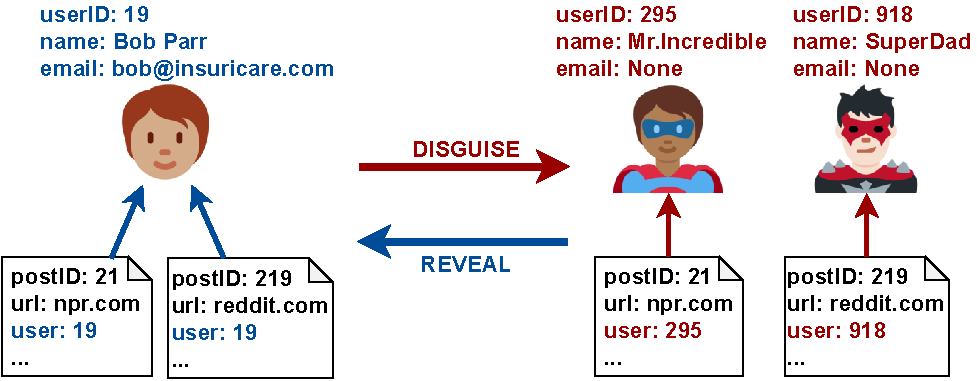
\includegraphics[width=0.47\textwidth]{img/disguises_new}

    \caption{Disguises move data (in this example, user Bob) from
             beteeen different \emph{guises}. Guises represent the
             same data, but with different privacy properties (\eg
             anonymization).}
    \label{fig:example}
\end{figure}

%
We propose \emph{data disguising}, a systematic approach to privacy
transformations that separates them from application code.
%
Data disguising reasons about \emph{disguises}, privacy transformations that
follow an organized structure.
%
Disguises are based on the observation that application data can take
different forms, some of which are identity-revealing while others are
privacy-preserving (to varying degrees).
%
%For example, a web application's database contents may assocate posts with
%an actual user as their author (an identity-revealing guise), or with
%one or more anonymous placeholder users (privacy-preserving guises).
%
A disguise transforms the database contents between these guises
(Figure~\ref{fig:example}).
%
%The structured nature of disguises allows a data disguising tool to
%automatically determine how to correctly compose multiple disguises, and to
%check that the end-state achieves the desired privacy properties.
%
%The tool uses the abstraction of \emph{per-user vaults}, which allow the tool to
%reintroduce destroyed data from prior disguises as necessary, while still ensuring that user data
%remains protected (\S\ref{sec:composition}).
%
%

%
An external data disguising tool reasons about and applies these disguises
based on the application's policy (a \emph{disguise specification}).
%
Application developers only need to invoke the tool's API to provide the
specification and to trigger individual disguises; the tool then performs the
necessary physical changes to the application's database.
%
These changes may include data removal, modification of contents, or
decorrelation by modifying references between objects.
%

\subsection{An Example Disguise}
\label{design:eg}
%
Consider disguising Bob when he deletes his HotCRP account.
%
Bob would prefer his papers and reviews to be unlinked from his identity.
%
HotCRP, on the other hand, would like to retain paper and review information that other users
find useful~\cite{hotcrp-privacy}.
%
An application developer can easily achieve both with disguises.
%A careful selection of edge and object transformations achieves both.
%

%
The application developer writes a short specification of the disguise.
%
Bob is unlinked from his
reviews via a predicated-transformation that decorrelates any reviews that reference Bob.
%
This transforms Bob into one unique user guise per review.
%
The disguise generates guise attribute values using suitable defaults;
%
in particular, HotCRP users' \texttt{disabled} attribute is set for the guises, ensuring that guises
have no permissions and never review papers.
%

%
Bob is linked to papers through conflicts, which can indicate coauthorship or a reviewer conflict.
%
These conflicts are not reassigned to the new guises, since preserved conflicts could reidentify Bob
as the likely author of a review. Thus, conflicts predicated on linking Bob to papers will be
removed.

%The disguise leaves all other edge types, ensuring that review and paper artifacts remain correctly
%linked: active reviewers still see the correct paper for their reviews, and active authors see the
%correct reviews for their papers, albeit potentially authored by anonymous, unlinkable guises of the
%original reviewer.
Unlike the current real-world HotCRP account deletion policy~\cite{hotcrp:privacy}, which deletes
all objects belonging to Bob, this disguise strikes a balance between decorrelating Bob's identity
from his reviews and papers, and maintaining useful information for other HotCRP users.
%
Furthermore, it is easy to imagine extending this disguise to automatically disguise Bob after some
time (\eg 2 years after the conference), protecting his future research career by hiding youthful
reviewing sins.
%

The tool disguises Bob when he invokes HotCRP account deletion. Bob provides his secret key to
decrypt and read from his vault, allowing the tool to retrieve and temporarily reverse any conflicting,
reversible transformations that would make Bob's deletion fail: in particular, it recorrelates any
of Bob's decorrelated paper conflicts and then properly removes them. (Because the conflicts are
removed, the decorrelation is not reapplied).  Bob wants his account deletion disguise to be
reversible, so after performing the specified disguise updates, the tool records each transformation
in the vault, re-encrypts the vault, and forgets the key.

\section{Our Current Data Disguising Framework}

We propose \emph{data disguising}, a systematic approach to privacy transformations
that separates them from application code.
%
We believe that data disguising systems will help support flexible privacy
transformations.
%
Data disguising represents privacy transformations as structured \emph{disguises}
that the application developer specifies to capture an application's privacy policies.
%
Applications invoke an external data disguising tool's API to apply disguises; the tool
interprets the specification and applies the necessary physical changes to the
database.
%
Data disguising offers mechanisms to handle interactions between disguises and
reversible disguises.
%in the form of automatically-generated \emph{revealing functions} stored in \emph{vaults}.

%
%In the following, we sketch one design for a data disguising framework.
%
%Some of the specific design decisions in this framework have alternatives that are worth
%investigating, and open research questions remain; we discuss these in \S\ref{s:disc}.

\subsection{Disguises: Structured Privacy Transformations}
\label{sec:disguises}

\begin{figure}[t]
    \centering
    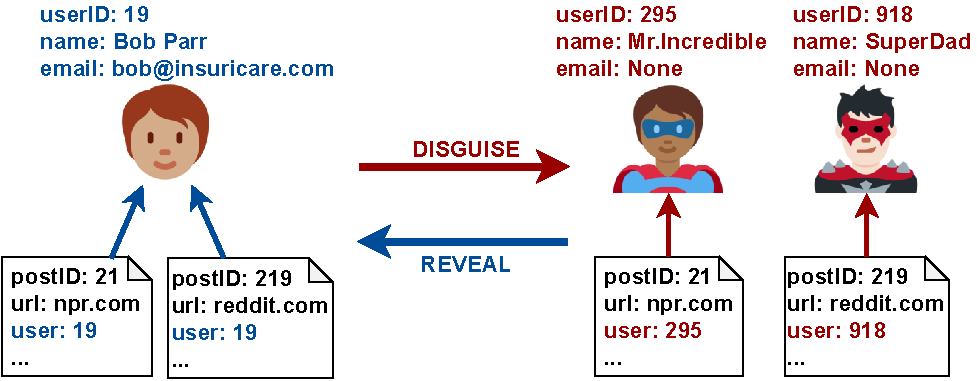
\includegraphics[width=0.47\textwidth]{img/disguises_new}

    \caption{HotCRP's user scrubbing disguise decorrelates Bea's reviews from Bea's identity while maintaining
    referential integrity using anonymous placeholders.}
    \label{fig:example}
\end{figure}

\begin{figure}[t!]
    \centering
    \footnotesize
\begin{lstlisting}[language=Rust]
disguise_name: "UserScrub",
user_to_disguise: $UID,
tables:
   ContactInfo:
      generate_placeholder: [
         ("name", Random),
         ("email", Default(None)),
         ("disabled", Default(true)),
         ..
      ],
      transformations: [Remove(pred: "contactId" = $UID)]
   ReviewPreference:
      transformations: [Remove(pred: "contactId" = $UID)]
   Review:
      transformations: [Decorrelate(
         pred: "contactId" = $UID,
         foreign_key: ("contactId", ContactInfo)
      )]
\end{lstlisting}
    \caption{Part of a HotCRP user scrubbing disguise specification. \texttt{\$UID} refers
    to the user invoking the disguise.}
    \label{fig:spec}
\end{figure}

%
The broad range and application-specific nature of privacy transformations poses a real
implementation challenge.
%
Most importantly, transformations must maintain the integrity of the application's data
in storage when applied.
%
For example, decorrelating users from their reviews could easily violate referential
integrity (\ie no dangling foreign keys) unless applied carefully.
%
%We believe that data disguising makes privacy transformations more manageable by
%separating them from application code, and
%
Data disguises' structured nature and automated application seeks to ensure this
property.
%

%
Data disguises are built on three fundamental transformation operations---data removal, object content
modification, and decorrelation by modifying references between objects---that can
capture and structure many desirable privacy transformations.
%
The application developer writes a disguise specification for each of the application's
privacy transformations.
%
This specification consists of predicated transformation operations on each table, which describe
how to transform objects that satisfy the predicate.
%
The data disguising tool takes the disguise specification and turns it into storage
operations that appropriately rewrite affected foreign keys.
%

%
Figure~\ref{fig:example} illustrates how the tool performs the example user
account deletion disguise for Bea, when given a specification like that in Figure~\ref{fig:spec}.
%
When her account is active, Bea's profile is associated with her true identity and her
reviews.
%
When Bea deletes her account, her reviews move to privacy-preserving
placeholders, making it seem as if a different user entered each of Bea's reviews.
%
This prevents an observer from correlating these contributions to expose Bea's identity,
but importantly preserves referential integrity.
%

%
%Disguises transform a guise by modifying it at per-attribute (\ie per-column) granularity, or
%splitting it into multiple guises in order to decorrelating from objects that reference it (via \eg foreign-key relationships).
%
%Guises can also be removed entirely.
%
%At any given moment, an application's data comprises a mix of identity-revealing guises
%and privacy-preserving ones. Disguises modify, split, and/or combine individual guises when triggered.

%-------------------------------------------------------------------------------
\subsection{Handling Disguise Interactions}
%\label{sec:composition}
%-------------------------------------------------------------------------------

Applications use disguises to achieve specific privacy goals, but this can be
complicated by interactions between different disguises.
%
Because disguises inherently reduce identifying information,
applying one disguise may change the outcome of future disguises applied on top of it.
%

%
For example, consider two desirable disguises in HotCRP: \gdpr and \ca.
%
\gdpr removes a user's account (\S\ref{design:eg}); \ca provides user privacy by
anonymizing all conference data.
%
These disguises touch the same data: applying \ca destroys information that \gdpr would
remove or transform if applied to an unmodified database.
%

%
In some cases, the disguises compose naturally---\eg there is no need to decorrelate
data that another disguise removed---but in others, the tool may need to access the
original data to meet the application's privacy goals.
%
%Even then, the necessary actions depend on the specific application:
%some applications may require that previously anonymized data still be deleted, while other
%applications may not.
%
Data disguising provides the infrastructure and mechanisms to reveal data to support
of disguise composition; however, automatically detecting when this is needed to
achieve application privacy goals remains an open challenge (\S\ref{s:disc}).
%To handle inter-disguise dependencies, a disguising tool relies on (1) the structured nature of
%disguises to
%statically determine whether disguises share dependencies, and (2) the key abstraction of \emph{user
%vaults}, namely per-user logs of disguise updates to that user's data.  User vaults solve the issue
%that disguises inherently destroy data necessary to correctly achieve the end-state of future
%disguises by providing a secure way to store the data. A disguising tool queries the user vault to
%temporarily restore destroyed data (\eg decorrelated foreign key relationships) in order to apply
%the disguise correctly.

%As shown in Figure~\ref{fig:tool}, a disguising tool sits next to the application, and queries the
%user vaults and the application database. The application performs disguises by invoking a
%disguising tool.

%-------------------------------------------------------------------------------
%\paragraph{Vaults.}
%-------------------------------------------------------------------------------
%
\textbf{Vaults} provide the infrastructure to reveal previously disguised data
when necessary.
%, either for temporary data for disguise composition, or for reversing a disguise entirely.
%
A vault is a storage location not accessible to application queries that stores
\emph{reveal functions} for applied disguises.
%
Applying these functions reveals the underlying data transformed by a disguise
(possibly temporarily).
%
%These functions are automatically produced by the disguising tool when a disguise is applied.
The disguising tool generates the reveal functions when applying a disguise, using
the specification and the disguised data.
%

%
Vaults admit various deployment models that have different security and privacy
properties.
%
%It remains important, however, that any configuration of vaults should not violate the
%guarantee that disguises indeed destroy data, from the viewpoint of the application and
%any users.
%
These include storing vaults in offline storage, which provides a modicum of security,
but makes access by the data disguising tool easy; or having vaults stored entirely by
some third party or locally by the user, with an API for disguise tool access.
%
The vault contents might be encrypted, and access might require explicit approval
by the user, who holds the private key.
%
\footnote{To protect against lost keys, the vault could be threshold encrypted with a private key
secret-shared~\cite{secretsharing} between the user, the web application, and a trusted third party
(\eg the EFF), so that the user can authorize the application and the third party to decrypt.}
%
Entries in a vault could also be configured to expire after some time; making the
corresponding disguises irreversible.
%

%
The vault deployment model can greatly affect the practicality of disguise
reversal.
%
For example, a reversible \gdpr must store reveal functions in per-user vaults
external to the application storage to be GDPR-compliant.
%
While it is reasonable to imagine accessing a single user's vault to reverse \gdpr in
this model, complete reversal of \ca would need to retrieve reveal functions from
all users' vaults, an infeasible task.
%
An alternative might be to provide multi-tier security: the first tier stores reveal
functions of non-GDPR disguises in a global vault accessible to the disguising tool
and application, while the second tier stores reveal functions from user-invoked
disguises in external, per-user encrypted vaults.
%
We imagine that exploring different vault designs will be an important part of
data disguising research.
%

%-------------------------------------------------------------------------------
%\paragraph{Revealing Data.}
%-------------------------------------------------------------------------------
%\lyt{I feel like this sticks out, but it is a reasonable part of our solution to handling disguise
%reversal.}
\textbf{Reverting disguises.}
%
Reveal functions also help with explicit disguise reversal (\eg a returning user): the
application invokes the disguising tool's API to revert a previously applied disguise.
%
This reversal permanently reveals data, restoring it to the application database.
%
However, other disguises may have affected the database contents in the interval between
the original disguising and the explicit reveal.
%
To ensure that any revealed data still respects other active disguises, the tool keeps
a persistent log of all disguises the application applied, and re-applies disguises from
the relevant log interval to the revealed data.
%

%
For example, reversal of \gdpr must avoid reintroducing identifiable reviews if \ca has
occurred since \gdpr was applied.
%
The data disguising tool would applying the relevant \ca anonymization operations to any
revealed data from \gdpr's reversal before making it visible the application.
%

%
Explicit application modifications to disguised data (other than deletion) are harder to
handle; the framework might prohibit them, or log them to the relevant vaults.
%

%\ms{OLD TEXT FOLLOWS}

\iffalse
%For example, Figure~\ref{fig:example} would include a specification that all email
%addresses be obfuscated in an anonymous manner for the user with name ``Bob Parr''.
%
%Transformations can either remove objects, or change objects into one or more guises.
%To create a guise from an object, developers specify how to transform attributes of the
%object (\eg table column values) into guise attributes (\eg changing email addresses).

%
%When writing a disguise, developers can reason about its
%specification in isolation; interactions between different disguises are handled by a disguising
%tool (\S\ref{sec:composition}).
%
%We assume that:
%\begin{enumerate}[nosep]
%  \item developers use their domain knowledge to write correct and complete disguises;
%      \lyt{should make clear that correct/complete is just operational? \eg doesn't mess up the DB}
%  \item application code handles the different guises appropriately (\eg in
%    displaying them); and
%  \item different guises of the same object have the same structure (\eg they can be
%    rows in the same table).
%\end{enumerate}
%
Developers choose how to create other guise attributes, selecting from among the following:
%
\paragraph{(1) Copy object content.}
%
Guises of the same object all share the object's attribute values.
%
If the attribute is a reference attribute (\eg a foreign key column), all guises will refer to the same object.
%
%
Copying allows developers to retain the object's content, without worrying about how to
synthesize attribute values for guises.
%
%However, this should only be chosen if guise attribute
%values cannot be generated, or if this attribute says little about the true identity of the
%entity.
For example, in Figure~\ref{fig:guises} the \texttt{darkmode} attribute is copied in
all guises.
%; the \texttt{darkmode} attribute reveals very little about the underlying user's
%identity.

\paragraph{(2) Generate new content.}
%
To create new attributes, developers specify whether the guise's value should be random,
a default value, or generated from the object's attribute value via a custom function (\eg hashing
the value).
%
Figure~\ref{fig:guises} illustrates an example of random (\texttt{name}) and default
(\texttt{active}) generated value attributes.
%
%
Creating new guise reference attributes (\eg new foreign key relationships) requires
creating a new guise for the referenced object in order to maintain referential
integrity;
the data disguise rewrites the reference to point to the new guise.
%
In Figure~\ref{fig:guises}, creating two user guises requires creating two
tag guises, and the tag guises' identifiers become the user guises' foreign keys.
%

\paragraph{(3) Copy object content, but only once.}
%
One guise copies the attribute value from the object, but all other guises generate new
values (as described above).
%
\texttt{notifs} in Figure~\ref{fig:guises} illustrates how the attribute is copied once.
%
This enables the application to retain the original object semantics (\eg a count of how many
users want notifications) without creating duplicates.
%



\begin{figure*}[t!]
    \centering
    \footnotesize
\begin{tabular}{@{}c|c|c|c@{}}
\textbf{User Transformation Spec} & \textbf{User Object} & \textbf{Guise 1} &
    \textbf{Guise 2} \\
\begin{lstlisting}[language=Rust]
"id":       IDAttribute,
"name":     Gen(Random),
"active":   Gen(Default(false)),
"darkmode": CopyAll,
"notifs":   CopyOnce+Gen(Default(false)),
"tag_id":   GenForeignKey,
\end{lstlisting}
    &
\begin{lstlisting}[language=Rust]
"id":       19,
"name":     BobParr,
"active":   true,
"darkmode": false,
"notifs":   true,
"tag_id":   11
\end{lstlisting}
&
\begin{lstlisting}[language=Rust]
"id":       295,
"name":     MrIncredible,
"active":   false,
"darkmode": false,
"notifs":   true,
"tag_id":   81483
\end{lstlisting}
&
\begin{lstlisting}[language=Rust]
"id":       918,
"name":     SuperDad,
"active":   false,
"darkmode": false,
"notifs":   false,
"tag_id":   15592
\end{lstlisting}
\end{tabular}
    \caption{Creating two guises of an example user (of a synthetic application schema).}
    \label{fig:guises}
\end{figure*}


%-------------------------------------------------------------------------------
\paragraph{Applying Disguises.}
%-------------------------------------------------------------------------------
A disguising tool applies disguises in a five-phase procedure:
\begin{enumerate}[nosep]
    \item \emph{Prepare}: execute the appropriate reveal functions of co-dependent,
        reversible disguises from the user vaults, if applicable (\S\ref{sec:composition})
        %reconcile any data dependencies between this disguise and prior disguises.
        %A disguising tool detects read-after-write dependencies between the new disguise's
        %predicates and prior disguises' updates, and, using entries in the vault, undoes any writes
        %that may affect the new disguise's predicates. As an optimization, vault entries recording
        %object removals need not be reversed.
        \item \emph{Read}: get all objects that satisfy (per-type) developer-specified predicates.
        \item \emph{Update}: modify, decorrelate, or remove objects read in step (2) according to the
        developer's specification.
    \item \emph{Record}: if the disguise is reversible, store per-user reveal functions for the
        disguise in the appropriate per-user vaults.
        A disguising tool must be able to determine which user vault should record each modification. This can be
        developer-specified, or rely on a set of heuristics (\eg assigning ownership by traversing,
        starting from each user, the application's object graph expressed in an object-relational
        model (ORM)~\cite{orm}, or implicitly via foreign keys).
        \item \emph{Finalize}: After applying the new disguise updates, the disguising tool
            redisguises any temporarily revealed data from earlier disguises.
\end{enumerate}

%Composed disguises should achieve an end-state that combines, in some way, the end-states achieved by each disguise when applied to the original application database in isolation.
%Correct composition of multiple disguises achieves an end-state equivalent to combining the
%end-states achieved by each disguise when applied to the original application database in isolation.
%
%If a prior disguise is reversible, then a disguising tool can use user vaults to ensure that this
%prior disguise does not affect \emph{which} objects are updated
%a future disguises.
%%In this case, a disguising tool allows developers to reason about multiple conflicting updates to
%the same object:
%regardless of when the disguises occurred, if one disguise removes an object that the other disguise
%modified, then the removal takes precedence.
%%
%
%However, if they both modify the same object attribute, a disguising tool establishes no precedence
%between the modifications and applies them in chronological order.  Alternatively, we can imagine
%that the developer could specify a partial ordering between modifications, or our framework could
%restrict the set of possible modifications and establish a precedence order within this set.
%
%If the prior disguise is not reversible, however, then the disguising tool could prevent future
%conflicting disguise application, or perhaps a-priori prevent the application of such non-reversible
%disguises that conflict with legally required disguises such as GDPR deletion \lyt{not sure what to
%put here? May also want to include something about developer assertions}
%%: a disguise will update all objects that it would have updated if performed on
%the original, undisguised state of application data.


\fi

%\section{Reasoning about Multiple Disguises}
\label{sec:composition}

Applications benefit from the ability to apply multiple disguises. For example,
\S\ref{sec:motivation} highlights two desirable disguises in HotCRP, namely \gdpr and \ca. \gdpr
provides user privacy by removing the user's data; \ca provides user privacy by anonymization.
As we observed, however, disguises may not be independent: applying \ca destroys information allowing \gdpr to properly remove the user's data.

Applications define an acceptable outcome after composing multiple disguises when they define their
privacy policy.
For example, HotCRP may require that \gdpr removes the invoking user's reviews completely, even when
applied after other disguises such as \ca.  Alternatively, HotCRP may accept a post-\gdpr outcome that either
anonymizes or removes reviews. 
The ability of the tool to achieve an acceptable outcome depends on both the application's privacy
policy and the reversibiility of the disguises (\ie do they discard reveal functions, or store
per-user reveal functions in user vaults?).

For example, assume HotCRP requires that a user's \gdpr disguise must \emph{remove} the invoking
user's reviews. If \ca allows per-user reveal functions to be stored in user vaults, then the
disguising tool can query the user's vault to temporarily recorrelate the user's reviews with their
identity before applying \gdpr for the user.  This allows the tool to remove the user's reviews when
\gdpr is applied, even if \ca has been previously applied.
%This requires the user to grant access to their vault.
%If one disguise removes an object that the other disguise
%modified, then the removal takes precedence.
%
%However, if they both modify the same object attribute, a disguising tool establishes no precedence
%between the modifications and applies them in chronological order.  Alternatively, we can imagine
%that the developer could specify a partial ordering between modifications, or our framework could
%restrict the set of possible modifications and establish a precedence order within this set.

However, if \ca is irreversible and the disguising tool \emph{discards} the reveal functions produced when executing \ca, then the tool cannot perform \gdpr while guaranteeing that \gdpr
removes all the user's originally owned reviews.  The right solution here is unclear: one
possibility is for the tool to a-priori determine (via, \eg static dependency analysis) the set of
irreversible disguises such as \ca that could prevent \gdpr from removing the user's reviews. This
analysis could be presented to the developer, providing a warning that the privacy policy may be
violated if \gdpr is applied after \ca.

If HotCRP's policy instead accepts that a user's \gdpr disguise can either remove \emph{or} anonymize the
invoking user's reviews, then the disguising tool can simply execute \gdpr on top of \ca and achieve
an acceptable state: any reviews missed by \gdpr would necessarily have been anonymized by \ca.
Thus, the tool can achieve HotCRP's privacy policy regardless of whether \ca discards or stores
reveal functions in user vaults.

\subsection{Reasoning about Complete Disguise Reversals}
Reasoning about multiple disguises is further complicated when disguises are intermixed with
disguise reversals.
%
For example, imagine that \ca and \gdpr both store reveal functions in user vaults. 
%
\ca followed by a user's \gdpr followed by the reversal of \ca should ensure that the deleted user's
reviews are still anonymized or removed (depending on HotCRP's specific policy for \gdpr).
Similarly, the user's \gdpr followed by \ca followed by the reversal of the user's \gdpr should also
ensure that the deleted user's reviews are anonymized.
To handle these scenarios, the disguising tool could keep a persistent log of all disguises performed by the
application; any disguises performed between a disguise's application and its reversal are 
applied to any reintroduced data. In the former scenario, \gdpr's removal would apply to any
recorrelated reviews; in the latter scenario, \ca's decorrelation would apply to any of the user's reintroduced reviews.

\lyt{This doesn't fit in well, but we should discuss it.}
Furthermore, vault deployment models greatly affect the practicality of complete disguise reversal. \gdpr
necessarily must store user vaults external to the application in order to be GDPR-compliant;
however, complete reversal of \ca requires retrieving reveal functions from every user's vault,
which is infeasible in a setting in which vaults live in external storage, encrypted with per-user keys.

%\section{An Example Disguise}
\label{design:eg}
%
Consider disguising Bob when he deletes his HotCRP account.
%
Bob would prefer his papers and reviews to be unlinked from his identity.
%
HotCRP, on the other hand, would like to retain paper and review information that other users
find useful.
%
An application developer can easily achieve both with disguises.
%A careful selection of edge and object transformations achieves both.
%

The application developer writes a short specifcation of the disguise. Bob is unlinked from his
reviews via a predicated-transformation that decorrelates any reviews that reference Bob.
%
This transforms Bob into one unique user guise per review.
%
The disguise generates guise attribute values using suitable defaults;
%
in particular, HotCRP users' \texttt{disabled} attribute is set for the guises, ensuring that guises
have no permissions and never review papers.
%

%
Bob is linked to papers through conflicts, which can indicate coauthorship or a reviewer conflict.
%
These conflicts are not reassigned to the new guises, since preserved conflicts could reidentify Bob
as the likely author of a review. Thus, conflicts predicated on linking Bob to papers will be
removed.

%The disguise leaves all other edge types, ensuring that review and paper artifacts remain correctly
%linked: active reviewers still see the correct paper for their reviews, and active authors see the
%correct reviews for their papers, albeit potentially authored by anonymous, unlinkable guises of the
%original reviewer.
Unlike the current real-world HotCRP account deletion policy~\cite{hotcrp:privacy}, which deletes
all objects belonging to Bob, this disguise strikes a balance between decorrelating Bob's identity
from his reviews and papers, and maintaining useful information for other HotCRP users.
%
Furthermore, it is easy to imagine extending this disguise to automatically disguise Bob after some
time (\eg 2 years after the conference), protecting his future research career by hiding youthful
reviewing sins.
%

The tool performs the disguise when Bob invokes HotCRP account deletion. To do so correctly, Bob
provides his secret key to decrypt and read from his vault. The tool retrieves and temporarily reverses any conflicting
transformations that would make Bob's deletion fail: in particular, it recorrelates any of Bob's decorrelated
paper conflicts and then properly removes them. (Because the conflicts are removed, the
decorrelation is not reapplied). After performing the transformations specified in the disguise, the
tool records each transformation in the vault, and re-encrypts it, forgetting the key.

%-------------------------------------------------------------------------------
\section{Prototype Implementation}
%-------------------------------------------------------------------------------
\label{sec:proto}
Our initial data masking system, \sys, consists of 5K LoC of Rust, and supports SQL queries as well
as \texttt{TRANSFORM [entity\_id]} and \texttt{REVERSE TRANSFORM [entity\_id]} queries.
\sys provides data masking in the context of applications that use SQL-based databases, and where
entities are schema tables and edges are foreign key relationships. 
%
This restriction is not fundamental: for example, we can imagine a data masking implementation that
additionally supports edges from \eg users to abstract, non-table entities such as ``country.''
%We show that \sys performs reasonably (Section~\ref{sec:perf}) for , and we plan to support
%eventually
%consistent, crash-recoverable transformations, sharding, and multicore parallelism.

If prompted, our prototype will record all transformations performed while data masking. This log can be
encrypted and stored in an additional table. The encrypting key can be kept by the application for
\eg content moderation transformations, or in the case of user unsubscription,
secret-shared~\cite{secretsharing} among the user, \sys, and a trusted third party so that the user
can retrieve a lost key without trusting the application or \sys. To undo the transformation, \sys
decrypts this log and reverses the modifications, restoring the affected portion of the entity graph
to its original state.

\iffalse
%-------------------------------------------------------------------------------
\section{Implementation}
%-------------------------------------------------------------------------------

\name introduces in-memory shim layer on top of a MySQL database, 
allowing \name to intercept and process queries sent by the application frontend. 
To amortize the cost of unsubscription and resubscription, \name preemptively creates, stores, and
links ghost parent entities to child entities if an update creates an edge that may be decorrelated.
\name builds in-memory materialized views on top of the underlying database, exposing ghost
entities only if the true entity has been decorrelated, and real entities otherwise. Updates
propagate to the materialized views when the underlying database is updated. \name answers
application queries using these materialized views, hiding the complexity of ghost entity and
decorrelation management.

\name is build in 5K LoC of Rust, and supports a subset of MySQL. \name adds \texttt{UNSUBSCRIBE
[user]} and \texttt{RESUBSCRIBE [user] WITH [user\_data]} calls to the query language.
\lyt{Should I mention details like query parsing, single-threaded?}

\subsection{Stored Data}
In addition to the original application data tables, \name stores a persistent mapping from entity
ID (EID) to a set of ghost IDs (GID). This mapping is cached in the shim layer for performance. Only
ghost entities that correspond to a true parent entity are stored in the mapping: auxiliary ghosts that are
created to introduce noise (reduce sensitivity), or to satisfy referential integrity---all their
children are also ghosts---are not linked to the real parent EID.

\name stores the in-memory materialized views for each datatable, using hashtables and btrees for
table indexes. An in-memory cache of the graph of parent-child entity key relationships built on
top of the views is also stored for unsubscription and resubscription performance.

Finally, \name stores a persistent and in-memory record of the hash of unsubscribed user EIDs 
and their removed application data to verify upon resubscription.

\subsection{Handling Normal Execution Queries}
\paragraph{Reads.}
Reads are answered by the materialized views. Because the materialized views are kept up-to-date with any application
writes, no queries to the underlying datatables are performed.
\lyt{I'm not sure if it's appropriate or interesting to put some of the MV query handling stuff
here? (Like processing joins, etc.)}

\paragraph{Inserts.}
When the application inserts an entity, \name first checks (using the developer-provided policy)
whether the entity is a child entity (i.e., it has a foreign key to another data table), and
whether the policy specifies that this child-parent key relationship should be decorrelated during
unsubscription. 

If so, \name preemptively creates a \emph{ghost parent} entity using the appropriate entity
generation policy, and adds this ghost to the parent data table. \name then saves the child
entity's real parent EID (the child entity's foreign key column value), and adds a mapping from this
EID to the new ghost parent GID.\footnote{\name assumes that the application does not violate
referential integrity, namely that any child entity inserted into the system will refer to a
corresponding parent in the database.} Finally, \name rewrites the child entity's foreign key
reference to correspond to this new ghost parent's GID, and stores the child into the datatable.

Note that generating the ghost parent may recursively generate a set of ghost ancestors for that
parent as well (to satisfy referential integrity). These ancestors are also added to the parent data
table.

The insert then propagates to the materialized view, inserting the entity with its real parent EID; queries that
select for this entity will not see any ghost entities. 

If the child-parent key relationship should not be decorrelated, or the inserted entity is not a
child, \name simply inserts the entity as-is into the datatable, and the materialized view is
updated with the entity.

\name also updates the parent-child entity graph with the new entity if the entity adds any edges
specified by the developer-provided policy. This graph is built on top of the materialized view, and
thus contains only those entities exposed by the materialized view to the application.

\paragraph{Updates.}
When the application updates an entity, \name again checks (using the developer-provided policy) whether
the entity is a child entity (i.e., it has a foreign key to another data table). 
If the entity is a child, and the policy specifies that this child-parent key
relationship should be decorrelated during unsubscription, then \name performs one final check of
whether the entity's parent key is one of the columns being updated.

If yes, then \name gets the current value of the entity parent key in the datatable: because \name
inserts only GIDs into the datatable for these decorrelatable child-parent links, this value 
corresponds to some ghost parent GID.
\name checks its ghosts mapping table for which real parent EID currently maps to this GID, removes
this current mapping, and updates the mapping so that the updated parent key value now points to
this GID.
\name updates all non-foreign key columns as normal, with values specified by the application.

If the updated entity is not a child of a decorrelatable edge, the update is performed without any
alterations.

Updates are propagated to the materialized view without modifying the values, so that application
reads only observe real parent entities.
\name also updates the parent-child entity graph if any edges between materialized view entities change.

\paragraph{Deletes.}
When the application deletes an entity, \name checks whether
the entity is a child entity (i.e., it has a foreign key to another data table). 
If the entity is a child, and the policy specifies that this child-parent key
relationship should be decorrelated during unsubscription, then \name gets the current value of the
entity parent key in the datatable, which must correspond to some ghost parent GID.
\name checks its ghosts mapping table for which real parent EID currently maps to this GID and removes
this mapping. \name also removes the ghost parent with this GID.

In all cases, \name removes the entity being deleted.
The deletion is propagated to the materialized view and removes the entity being deleted; the
parent-child entity graph is modified appropriately.

\subsection{Handling Unsubscription}
\paragraph{Traversal.}
\name is given the top-level entity type and EID to be decorrelated (typically a user and a user ID).
\name then performs a (depth-first) traversal of the parent-child entity graph built on top of the materialized
views. 

\name stores all the children entities traversed during decorrelation for post-processing, and
handles parent-child edges as follows:

If a parent-child edge has a no-decorrelation-retain policy, \name does nothing; if a parent child-edge has a
no-decorrelation-delete policy, \name removes the child entity and recursively removes all of its
descendants. 
\lyt{TODO: \name should apply the ghost generation policy to the parent node (replacing it with a ghost) for retain policies if a ghost generation policy exists.}

For every parent-child edge with a decorrelate policy, \name looks up the parent EID in the
EID to GIDs mapping, saves the corresponding GIDs, and removes the mapping (both persistent and
cached).
\name then updates the child entity in the materialized view to point to a ghost entity instead
than the real parent (who is being decorrelated) by choosing one of the corresponding GIDs for this
parent and updating the child's parent key with this GID.  The parent-child entity graph is updated
accordingly to include the ghost parent (note that this does not affect the traversal, which only
traverses parent-child edges).

If a parent-child edge has a no-decorrelation-sensitivity policy, \name stores the edge for
post-processing.

\paragraph{Sensitive Parent-Child Edges.}
Post-traversal, \name considers its collected set of sensitive edges. For every unique parent,
\name counts how many children attach to the parent for each distinct edge type (e.g,\ for a
particular tag, how many stories are linked to this tag, how many comments are linked to this tag,
etc.). For each child count $n$, and with an edge type sensitivity threshold of $\sigma$, 
\name generates $n / \sigma$ ghost entities of that child type, all of which have an edge to the parent.
These ghost entities are inserted both into the materialized views, and into the underlying
datatables; however, because they do not correspond to real entities, EID to GID mappings are not
stored. 
If \name finds no ghost generation policy for the child entity type, \name instead recursively
removes the child and its descendants.

\paragraph{Handling Child-Parent Edges.}
Next, \name considers child-parent edges from the collected set of traversed children to parents
not seen during \name's traversal. If an 
edge can be decorrelated, \name rewrites the materialized child parent key to one of the parent
ghost GIDs. The ghost GID is retrieved by querying the parent's EID to GIDs mapping, the
corresponding ghost parent is added to the materialized view,
and the mapping from parent EID to GID is subsequently removed. These steps ensure that the
materialized view reflects that the link between the child and the original parent has been
decorrelated.

If an edge has a delete policy, the child and its descendants are removed; if an edge has a retain
policy, nothing is done. 
%
\lyt{TODO: for retain policies, the ghost generation policy should be applied to the child node if
the ghost generation policy exists.}

If an edge $e$ has a senstivity threshold,
\name counts $N_{all}$, the total number of edges of the same edge type as $e$ that connect to $e$'s parent.
\name then counts $N_{sensitive}$, the number of these edges that connect to children that were traversed by \name during the
first decorrelation step (this number includes $e$).
If $e$'s edge type has sensitivity threshold of $\sigma$ and $N_{sensitive} / N_{all} > \sigma$,
\name generates $\lceil N_{sensitive}*\sigma\rceil - N_{all}$ ghost entities of $e$'s child type, all
of which have an edge to $e$'s parent.
As before, these ghost entities are inserted both into the materialized views, and into the underlying
datatables; however, because they do not correspond to real entities, EID to GID mappings are not
stored. 
If \name finds no ghost generation policy for the child entity type, \name instead recursively
removes the child and its descendants.

\paragraph{Decorrelated Entity Removal and Return Values.}
Finally, \name removes any completely isolated entities, namely any real entities that have no
descendants and are linked to only ghost (or no) parents. A completely isolated entity has either been swapped
out for a single ghost entity (in the case of a retained edge), or replaced by several ghost
entities, one per each decorrelated edge.

\name returns to the unsubscribing user (1) the removed parent EID to GIDs mappings, (2) any
completely isolated (and removed) entities,
and (3) the GIDs of any ghosts generated during sensitivity checks or to replace real
entities at the ends of retained edges.

To ensure that the end user cannot tamper with their application data while unsubscribed, \name saves
persistent and in-memory copies of the hash of the top-level entity EID and the returned data to
check upon resubscription.

\subsection{Handling Resubscription}
\name is given the top-level entity type and EID to be resubscribed, along with the data returned
from a prior unsubscription.
\name verifies that the hash of the EID and data matches that from the latest unsubscription of
this entity.

\name first re-inserts the completely decorrelated entities that were removed during unsubscription
into both the datatables and materialized views. 

Next, for all removed parent EID to GIDs mappings, \name reinserts these mappings into the
persistent and cached EID to GIDs mapping.
\name then removes the corresponding ghost entities for all GIDs and any ghost ancestors of these
GIDS from the materialized views; note that these ghosts still remain present in the
persistent data tables for future unsubscription.
\name then updates all materialized children of these removed ghosts with the original parent EID. Looking up the relevant
children is facilitated by the in-memory entity graph. 

Finally, \name removes any
ghost entities from the datatables and materialized views that were created during unsubscription to
lower sensitivity.

\subsection{Handling Crashes and Recovery}
Upon a crash, the in-memory materialized views are rebuilt from the underlying datatables and ghost
mapping. Any datatable entities without parents are simply reinserted into the appropriate
materialized view. 

If a datatable's entities have parent entities, the parent foreign keys may be ghost parent GIDs. 
This can happen for two reasons: 1) these child-parent edges can be decorrelated, and so ghost
entities had been preemptively created in the datatable; or 2) these are ghost entities created to
add noise to sensitive correlations during an unsubscription. 

For each entity with ghost parent GIDs, \name checks whether a mapping
from a real parent EID to the parent GID exists in the persistent EID to GIDs mapping. 
If such a mapping exists, then the real parent entity should be exposed to the application because
the parent or its ancestors have not yet unsubscribed: \name inserts the child entity with the real parent
EID into the materialized view.

Otherwise, if no mapping exists, then the ghost parent was generated during an unsubscription, and
the top-level entity has not yet resubscribed. \name thus exposes the ghost entity by inserting the
unmodified child entity with the parent GID into the materialized view.
Note that this may link a child entity with a \emph{different} ghost user than initially decided
during unsubscription (where any one of the ghosts corresponding to the real parent could be used as
a ghost parent for any child). 
\lyt{I think this can also be avoided by updating the MV entities with GIDs in monotonically
increasing order, since this is how they would have been inserted into the underlying database. It
also doesn't seem that important.}

The parent-child graph is constructed appropriately on top of the materialized view, and the EID to
GIDs mapping cache repopulated.

\lyt{TODO: Unsubscriptions and resubscriptions should be logged so that we can determine if they've
completed or not upon crashing. Eventual consistency for persistent / MV state in unsub/resub.}
\fi

%%%%%%%%%%%%%%%%%%%%%%%%%%%%%%%%%%%%%%%%%%%%%%%%%%%%%%%%%%%%%%%%%%%%%%%%%%%%%%%%%%%%%%%%%%
\section{Evaluation}
\label{s:eval}
%%%%%%%%%%%%%%%%%%%%%%%%%%%%%%%%%%%%%%%%%%%%%%%%%%%%%%%%%%%%%%%%%%%%%%%%%%%%%%%%%%%%%%%%%%i

%
Our performance evaluation focuses on the Lobsters, WebSubmit, and HotCRP applications
from our case studies.
%
We seek to answer the four questions:
%
\begin{enumerate}[nosep]
 %
 \item Does \sys meet its security goals and provide meaningful guarantees to users?
   (\S\ref{s:eval-security})
 %
 \item How expensive are core \sys interactions, \emph{viz.}\ disguising, revealing, and
   operations over disguised data? (\S\ref{s:eval-ops})
 %
 \item How much does application latency and storage use increase when an application
   uses \sys? (\S\ref{s:eval-res})
 %
 \item How do disguise and reveal actions impact the performance of concurrently executing,
   normal application requests by other users? (\S\ref{s:eval-conc})
 %
\end{enumerate}
%
All benchmarks run on a 40-core server with Intel Xeon E5-2660 v3 CPUs and \note{XX} of RAM
running \note{Arch Linux XXX}.
%
We use the MariaDB RDMS for application data storage, but store all databases on \fn{tmpfs}
to avoid confounding factors related to persistence.
%

\subsection{Security Evaluation}
\label{s:eval-security}

%
\sys secures disguise records by encrypting them with the public key of a principal $p$.
%
The corresponding private key for $p$ is on the client device and unavailable to the
application and \sys until the client provides it as part of an operation over data
under disguise.
%
Therefore, principals who remain inactive or only perform normal application operations
that access the plaintext application DB always enjoy full privacy for their data under
disguise, as an attacker who compromises the server cannot obtain their private key.
%

%
\sys uses locators to hide which disguises the application applied to which
principals' data.
%
A disguise creates \lcapa{pd} for disguise $d$ applied to principal $p$, and links it
to the disguise's bag of ciphertexts via an index, \lcapa{pd}$\to$ bag, in \sys's
public metadata.
%
The locator itself is a random byte string and does not contain $p$ or $d$, and
only the client has knowledge of the $(p, d)$ that \lcapa{pd} corresponds to after
the disguise completes.
%
Therefore, the the state of the index contains no metadata that lets the attacker
identify $p$ or $d$.
%
While an attacker can learn that $n$ records exist for \emph{some} $p$ and $d$ by
inspecting the index and bags, they cannot identify \emph{which} $p$ or $d$.
%

%
Because \sys stores locators from disguises over pseudoprincipal-owned data as part
of its pseudoprincipal metadata, \sys's disguise composition leaks that \emph{some}
number of disguises have applied to pseudoprincipal $q$.
%
However, these locators are encrypted with $q$'s private key, which is only accessible
by decrypting a bag protected by another principal's private key, a chain that extends
back to some natural principal $p$.
%
This prevents an attacker from finding out which bags belong to $q$, and therefore
also hides which bags correspond to natural principals' data.
%
Because $q$ is dissociated from the natural principal $p$ that speaks for $q$
(possibly via intermediate principals), the attacker cannot determine if natural
principal $p$ ever existed, nor if they have any data in \sys.
%

%
If an attacker compromises the server at time $t$, they can harvest any private key
that a client provides for operations after $t$.
%
The attacker can therefore reveal all current data under disguise stored in \sys and
encrypted with this private key.
%
Likewise, when a client provides $(\lcapa{pd}, p, d)$ to operate over data under disguise,
the attacker learns the correspondence between \lcapa{pd} and $(p, d)$.
%
But this merely makes the attack more efficient, as the attacker can already discover
$p$'s disguise history by attempting to decrypt all bags with $p$'s private key.
%
However, provided that the application deletes ciphertexts from \sys after revealing
the data, the attacker cannot gain access to any previously-revealed data that users
subsequently deleted from the application database.
%
\sys makes no guarantees for users who actively use data under disguise after
compromise, but always protects inactive users.
%

%
After a compromise occurs and is detected, users who performed operations on data
under disguise and whose private keys might have been compromised must start using new
keys.
%
This is easy: the application tells the client to generate a new key pair, and then
calls \fn{RegisterPrincipal} to register the natural principal's new public key with
\sys.
%
Future disguises now use this public key; \sys could also re-encrypt existing data
under disguise, but our prototype does not do so, as this data is already potentially
compromised.
%
A conscientious user might change their keypair for the application on a regular basis
to protect their data against undetected compromises.
%

\subsection{Performance of \sys Operations}
\label{s:eval-ops}

%
Next, we measure \sys's performance using disguises from our three case study
applications: WebSubmit, Lobsters, and HotCRP.
%
For each application, we measure the latency of normal operations as well as
privacy transformations.
%
In order to measure the extra cost added by \sys's cryptographic operations,
we implemented a manual, irreversible version of each privacy transformation,
as a developer would, by directly modifying the application database, and
measure its latency.
%
\sys allows applications to provide additional functionality, such as account
restoration and editing data under disguise, and we measure the latency of these
operations too.
%
A good result for \sys would show no overhead on normal application operations,
competitive performance with manual privacy transformations, and reasonable
latencies for data-revealing operations (\eg a few seconds for account
restoration).
%

\begin{figure}[t]
    \centering
    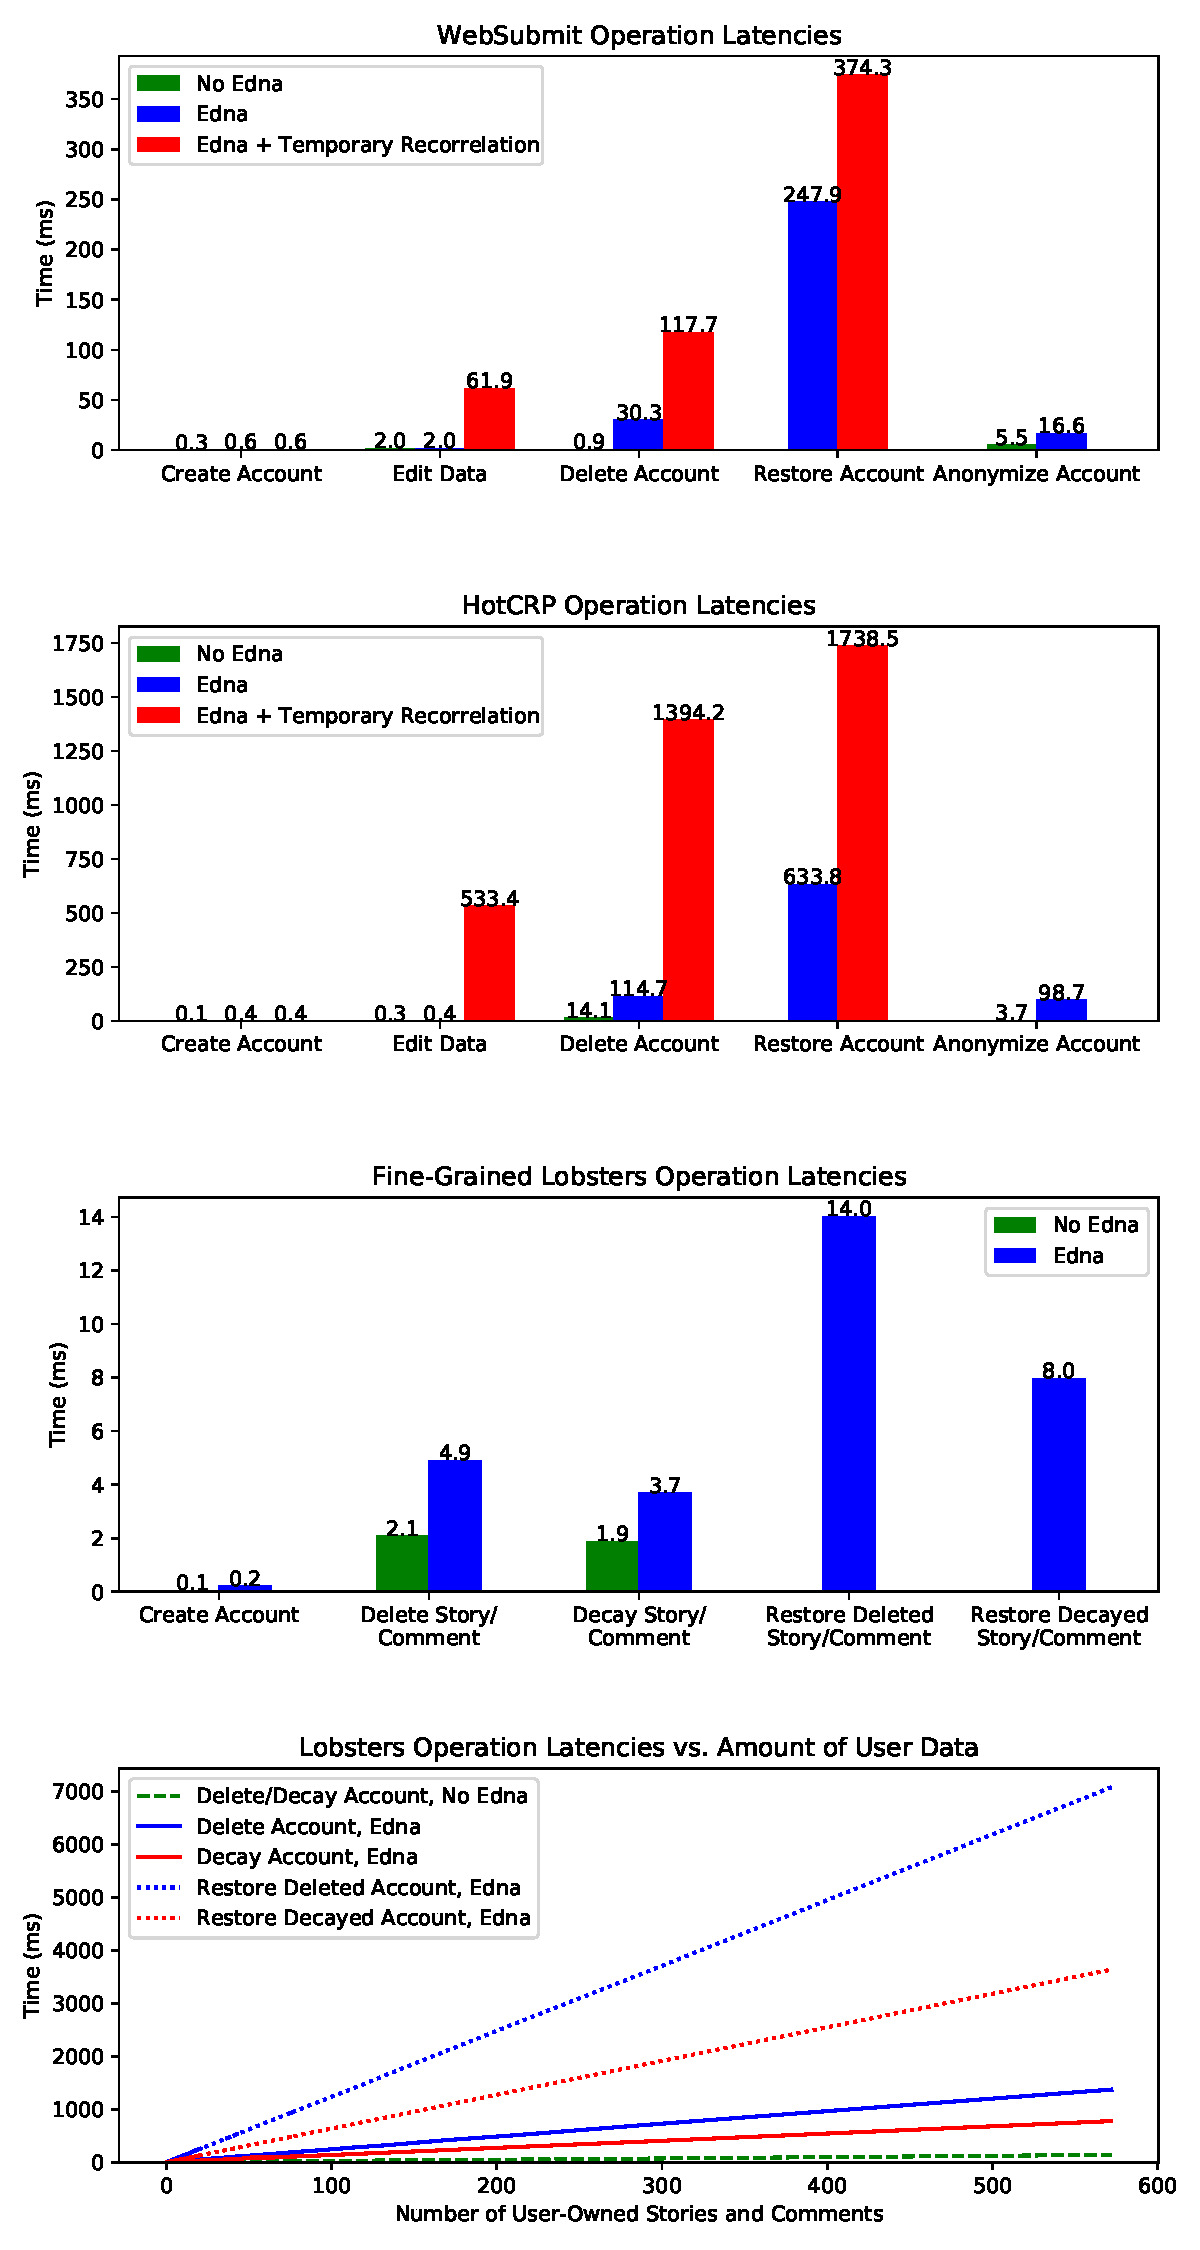
\includegraphics[width=0.5\textwidth]{figs/client_op_stats}
    \caption{Latencies of disguise-related actions when implemented manually by the
    application developer without \sys, and with \sys.
    Each bar shows the median latency; ranges indicate the 5th to 95th
    percentile latencies.}
    \label{fig:client_opstats}
\end{figure}

\begin{table*}[h!]
\begin{center}
\begin{tabular}{ c c }
\textbf{DB Op} & \textbf{Time (ms)}\\
\hline
Update DB Row & 0.1\\
Select DB Rows & 0.2\\
Remove DB Rows & 0.2\\
Reveal Deleted Row (DB Select + Insert) & 0.2 \\
Create + Register Principal & 0.1\\
\end{tabular}
\quad
\begin{tabular}{ c c }
\textbf{Crypto Op} & \textbf{Time (ms)}\\
\hline
Generate Keypair & 301\\
Encrypt SpeaksFor Record & 0.4\\
Decrypt SpeaksFor Record & 3.0\\
Encrypt Diff Record & 0.3\\
Decrypt Diff Record & 3.0\\
\end{tabular}
\end{center}
\caption{Amount of time required to run different operations required to apply and reveal disguises.}
\label{tab:opstats}
\end{table*}

\paragraph{WebSubmit.}
%
We run WebSubmit benchmarks with a database seeded with 2,000 users, 20
lectures with four questions each, and an answer for each question for
each user (160k total answers).
%
This might correspond to all classes in a department, or to a large AI class.
%
We measure end-to-end latency, which includes request processing in WebSubmit,
\sys's operations, and the response to the client.
%
The amount of data under disguise is constant across users, so we would expect
low variance in the results.
%

%
Figure~\ref{fig:websubmit-ops} shows the median latency for two normal operations
(creating an account and editing unanonymized data), two disguises (delete account
and anonymizing an account), and two operations over data under disguise (editing
anonymized data and restoring the account).
%
Normal operations have comparable latencies with and without \sys.
%

%
\sys's disguise-based account deletion takes 2.9ms, \vs 0.9ms in the manual
baseline.
%
This makes sense, as \sys encrypts database diffs and speaks-for records, while
the baseline only deletes data from the application DB.
%
The difference is greater for account anonymization, where \sys takes 10.8ms,
while the baseline takes less than 0.1ms.
\ms{why?}
%
Finally, \sys enables operations over data under disguise, which are impossible in
the baseline; these take 10.2ms and 21ms, well within acceptable interactive
latencies for web applications.
%
The simplicity of WebSubmit's disguises---which touch at maximum two database
tables---lead to fairly low latencies even for involved operations such as
restoring a deleted account (21ms).
%

\paragraph{HotCRP.}
%
We run the HotCRP experiments on a database seeded with 450 total users (50 of
whom are PC members), 450 papers, and four reviews and four comments per paper,
distributed evenly among PC members.
%
The benchmark measures the server-side latency to perform disguising and
application operations.
%
HotCRP supports the same disguise-related operations as WebSubmit.
%

HotCRP reviewers have slightly more variable amounts of data \lyt{TODO?} depending on the
assignment of papers to reviewers. HotCRP's disguises are far more complex than
WebSubmit's, touching 12 tables, and performing a mix of deletions and
decorrelations, leading to higher median latencies in general, even for the baseline.


\paragraph{Lobsters.}
%
We run Lobsters benchmarks on a database seeded with 14.5k users, which
is the late-2021 size of the real Lobsters site.
%
These users have \note{40k} stories, and \note{120k} comments with votes;
stories, comments, and votes are distributed among users according to
statistics from the actual Lobsters deployment~\cite{lobsters-data}.
%
The benchmark measures server-side latency of disguising and application
operations.
%

Lobsters supports account creation and deletion/restoration as well, but has account decay (and
subsequent restoration) instead of account anonymization.  It does not support editing anonymized
data (accounts can be restored in order to edit decorrelated data). In these benchmarks, we measure
the cost of GDPR-compliant account deletion and restoration.


Lobsters users' amount of data follows a skewed distribution, with most of the 5000 users
having fewer than 10 stories and comments, and a handful of users having over 300 stories and
comments. Lobster supports more complex disguises than WebSubmit and HotCRP,
touching 15 tables, and performing a mix of deletions, decorrelations, and modifications. This leads
to a higher latency as the amount of user data grows comparable to that of users in HotCRP and
WebSubmit.

\note{XXX old, unedited text follows. Malte is editing here.}

\paragraph{Drill-Down.}
%
Latency-critical tasks such as editing (unanonymized) data or
creating an account are largely unaffected by \sys.
%
To explain these costs, we break them down into fine-grained operations shown in
Table~\ref{tab:opstats}: every disguise action requires some DB operations and,
if using \sys, may require cryptographic operations.

\textbf{Creating an account} with or without \sys performs a database insert. Using \sys additionally
requires registering the new user as a principal, which assigns the user a (pre-generated)
private-public key pair, stores metadata about the new principal's key in \sys's storage, and
returns the corresponding private key to the application.
Using \sys thus incurs only the cost of an extra database operation, since the high cost of key
generation is taken offline.

\textbf{Editing data} with or without \sys simply performs database updates. Editing anonymized
data, however, requires \sys to decrypt (with the client-provided decryption capability) \emph{all}
speaks-for records at the client-provided locator until it finds a speaks-for record linking the
client to the currently-owning pseudoprincipal.  For example, if anonymization of a user account
generates 20 speaks-for record ciphertexts at the same locator, then editing anonymized data may
perform up to 20 decryptions to determine which pseudoprincipals the client can act for.

\textbf{Account deletion or data decay} with or without \sys performs the same database operations
to remove, modify, or anonymize data. \sys incurs increased costs by additionally encrypting and
inserting one diff record for each deleted or modified object, and one speaks-for record for each
anonymized object.

\textbf{Account restoration} is only possible with \sys. \sys decrypts a record for each
piece of modified/removed/anonymized data, and performs database checks to ensure the data can be restored
(\eg that the corresponding lecture of an answer to reinsert still exists). If the checks pass
(which they do in this benchmark), \sys restores the data stored in the diffs.

\textbf{Anonymization} with or without \sys generates one pseudoprincipal per object to anonymize
(\eg answers for lectures in WebSubmit, or reviews in HotCRP). Anonymization selects the relevant answers
to anonymize, generates new pseudoprincipals, and performs DB queries to insert new pseudoprincipals
and to update objects to point to these new pseudopricipals (\eg updating foreign keys).
\sys incurs increased costs by additionally generating per-pseudoprincipal speaks-for records, and
encrypting and storing these speaks-for records with the appropriate public keys.

\begin{figure}[t]
    \centering
    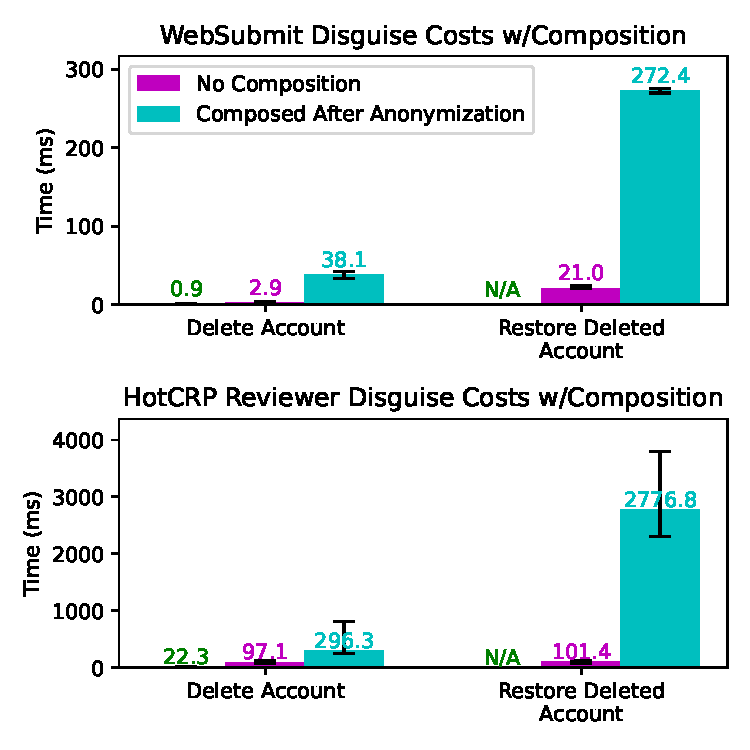
\includegraphics[width=0.45\textwidth]{figs/composition_stats}
    \caption{Latency of account delete and restore before anonymization vs. composed after anonymization.}
    \label{f:composition}
\end{figure}

\begin{figure*}[t]
    \centering
        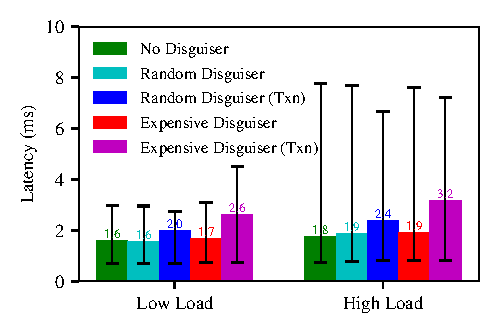
\includegraphics[width=0.45\textwidth]{figs/lobsters_concurrent_results}
        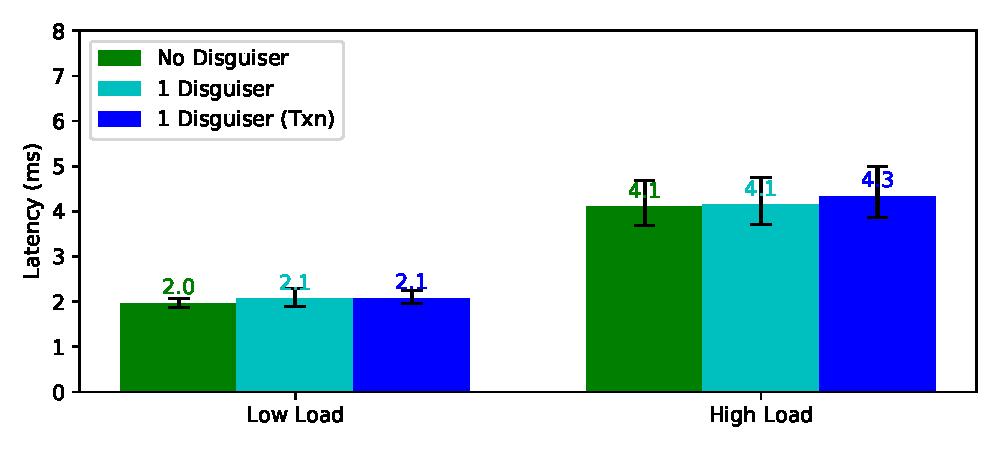
\includegraphics[width=0.45\textwidth]{figs/websubmit_concurrent_results}
    \caption{Impact of continuously applying and revealing account deletion disguises (non-transactional and transactional) on users concurrently running
    normal application operations. We show the median latency; ranges indicate the 5th to 95th
    percentile latencies.
    \textbf{Left (Lobsters)} tests the normal Lobsters traffic in the presence of an expensive
    disguiser (owning >6000 data objects) and a cheap disguiser (ownering <10 data objects). Even an expensive disguiser has minimal impact when user load is low; however, the impact increases as the server load increases, and if the
    disguise is transactional.
    \textbf{Right (WebSubmit)} tests an adversarial, write-only user workload of edits that
    modify the same table. All users have approximately the same amount of data (4 answers for 20
    lectures), and one user is chosen to continuously delete and restore their account. Here,
    disguising has minimal impact on latency even at high load.
    }
    \label{fig:concurrent}
\end{figure*}

\textbf{Composing Deletion After Anonymization.}
\lyt{TODO}
Account deletion post-anonymization requires \sys to perform temporary recorrelation find data of
pseudoprincipals that the user is authorized to remove along with their account. \sys incurs latency
increases from decrypting all speaks-for records of the user, and from performing the deletion or
modification queries for each discovered pseudoprincipal (in addition to the original user).

Account restoration may also restore pseudoprincipal-associated data, which requires temporary
recorrelation to access to pseudoprincipal-associated records produced from the account deletion.
\sys thus additionally decrypt speaks-for records for all pseudoprincipals of the user, which causes
the the increase in latency.\lyt{Numbers?}

%%%%%%%%%%%%%%%%%%%%%%%%%%%%%%%%%%%%%%%%%%%%%%%%%%%%%%%%%%%%%%%%%%%%%%%%
\subsection{Resource Use}
\label{s:eval-res}

Each generated pseudoprincipal adds an additional row to the users table in WebSubmit; \sys also
stores public-key metadata for each principal (and pseudoprincipal), and (in-memory) encrypted
ciphertexts for records.  Clients keep track of capabilities and locators that are emailed to them in
the form of URLs that allow for account restoration or post-anonymization editing.

%%%%%%%%%%%%%%%%%%%%%%%%%%%%%%%%%%%%%%%%%%%%%%%%%%%%%%%%%%%%%%%%%%%%%%%%
\subsection{Impact on Normal Application Use}
\label{s:eval-conc}

Figure~\ref{fig:concurrent} shows the impact of concurrently-running disguise actions on the latency
of normal application operations.

We first test the impact of disguising in Lobsters. We first achieve ~80\% CPU load by running
30 threads that model production Lobsters traffic. These threads simulate performing different
Lobsters operations (\eg loading the front-page, posting stories) according to measured access
frequencies and popularity distributions in production\lyt{CITE}. In this workload, 85\% of all
operations are front-page loads, which fetching stories and vote counts.

An additional number of threads simulate disguising users: these users (in the worst-case) decide to
simultaneously delete their account (\eg in response to some social media campaign). At some later
point in time, these users decide to come back and (in the worst case) simultaneously restore their
accounts.
We observe that even when the number of disguisers increases to 100, the latency of normal Lobsters
operation remains unaffected.

We then test an adversarial, write-only workload with WebSubmit. As a baseline, we achieve ~60\% CPU
load by running 100 threads that each continuously edit a user's lecture answers with 250-500ms
pauses between edits. This write-heavy workload achieves particularly high contention because all
edit queries modify the same database table; MySQL uses table-level locking for \texttt{MEMORY}
tables.

We then add an additional number of threads to simulate simultaneously disguising users.  While
fewer than 16 users disguising themselves at once has minimal impact on edit latency, 30 users doing
so causes spikes up to 4000ms.  These spikes come in pairs, with the larger second spike in the pair
coinciding with concurrent revealing (and the first of the pair coinciding with disguising);
revealing has greater impact due to its higher latency and compute costs.
%
Record batching improves these results by reducing the load generated by disguise actions: latency
spikes decrease to under 1500ms.

While we focus on normal application operation latency, we note that
disguise operation latency increases proportional to the overall system load (\eg due to MySQL’s
table-level locking). But this is acceptable, as disguises aren't time critical; in practice, they
still complete within a few seconds even at 60-80\% system load.
%
What matters is that normal application requests have acceptably low latency even in the presence of
disguising, which we achieve under realistic workloads (largely reads, with queries dispersed among
tables). If the workload becomes adversarial, \sys can prevent normal operation latency spikes by
rate-limiting disguise actions.

\section{Discussion}

\lyt{Should we note somewhere that pseudoprincipals and recursive disguising are why we need asymmetric
crypto; otherwise, we could just send the symmetric key to the original user being disguised?}

\lyt{
An alternative design might remove encrypted records completely (and \eg store them in external per-user
vaults or email them to the client).
This leaves no trace in \sys or the application, and would prevent the attacker from learning
anything. However, this places a large burden on the client.
Maybe put this in future work?
}

\ms{Hiding bag sizes -- very expensive, as would need to pad to max user data size, or add noise
proportional to that. Likely impractical.}

%-------------------------------------------------------------------------------
\section{Related Work}
%-------------------------------------------------------------------------------
\label{sec:related}

%
Protecting personal data in web services is a long-standing research direction.
%
\textbf{Decentralized platforms} such as Solid~\cite{solid}, BSTORE~\cite{bstore},
Databox~\cite{databox} and others~\cite{diy, amber, oort, w5, blockstack}
seek to put data directly under user control.
%
These systems give users power to control access, and often delete or modify, their
own data, but they burden users with maintaining infrastructure, typically lack the
capacity for useful application features based on server-side compute, and they break
the current, ad-based application revenue model.
%
In contrast, data disguising helps application developers support privacy
transformations without changing the application data model or business model,
and allows today's server-side processing.
%

%
Other platforms attest that server-side processing respects
\textbf{user-defined policies} over their data, via cryptographic means~\cite{zeph}
or systems security mechanisms~\cite{riverbed}.
%
The application functionality is typically restricted, in terms of the feasible
operations (\eg additively homomorphic ones) and in whether data with different policies
can be combined.
%
Data disguising only provides assurances about data privacy after the application has
disguised the data, but in exchange allows unrestricted application functionality
without any overhead.
%

%
Other systems enforce developer-specified \textbf{visibility and access control policies}
based on information flow control (IFC)~\cite{static, jeeves, jif, hails, ifdb},
authorized views~\cite{oracle} or per-user views~\cite{multiverse}, and rewriting database
queries~\cite{qapla, sieve}.
%
Data disguising transforms the actual data stored, and, unlike these systems, protects
against full server compromise.
%


%
New privacy laws have led researchers to propose \textbf{database designs
for privacy compliance}.
%
These databases track the owner of data objects and erase them on user request, compliant
with \eg the GDPR.
%
They either modify the data layout~\cite{usershards} or use fine-grained information flow
tracking (IFC) to determine PII propagation and restrict access~\cite{schengendb}.
%
Data disguising can be employed for GDPR compliance, but supports broader privacy
transformations that go beyond deleting PII, and requires no ownership tracking or
fine-grained IFC.
%

%
\textbf{Systems for data deletion}, on the other hand, specifically focus on the
challenge of correctly removing a user's to provide them with post-deletion
privacy.
%
While cryptographically-guaranteed deletion is difficult and expensive~\cite{vanish},
practical systems that help developers get deletion right exist.
%
DELF~\cite{delf}, a framework for data deletion at Facebook helps developers write
correct data deletion code, and uses annotations on application edge and object types
to specify a deletion policy.
%
DELF focuses only on data deletion, while data disguising targets broader privacy
transformations, including decorrelation and anonymization.
%
Sypse~\cite{sypse} pseudonymizes user data and partitions personally identifying
information (PII) from other data.
%
Like data disguising, Sypse's design is application-oblivious, and leaves
the specification of what counts as PII to the application.
%
Instead of constantly maintaining data partitions (as Sypse does), data disguising
adapts the application database on disguising and stores encrypted data to
potentially later reveal it.
%

%
Our work shares some ideas with \textbf{encrypted storage systems}.
%
However, the deployment scenarios for these systems assume that all data is
encrypted, which imposes overheads on normal operation and requires application
functionality to live on the client.
%
Support for arbitrary and fully-oblivious operation over encrypted data would
be ideal, but while there is encouraging recent progress on search over encrypted
data and oblivious key-value stores~\cite{dory, snoopy}, the cost is too high for
practical web services.
%
However, data disguising has a similar threat model to CryptDB~\cite{cryptdb},
Mylar~\cite{mylar}, or Keybase~\cite{keybase}, and protects confidentiality of
data under disguise against similar server compromises.
%
Data disguising encrypts only users' data currently under disguise, but is
efficient and still protects inactive users' privacy.
%

%
%Finally, privacy-enhancing techniques like $k$-anonymity, $l$-diversity, and
%differential privacy~\cite{dataminingmodels, differential} can complement
%data disguising.
%%
%Disguises might add differential privacy noise to
%data left in the application DB, for example.
%


%---------------------------

\iffalse
Key ideas:
    pseudonymization
    data partitioning
    synthetic data

Similarities:
- privacy guarantees weaker than DP, no constraints on queries
- pseudonymization --> overwrite a portion or all of data for individual, difficult to reassociate
    only a small fraction of data?
    breaking up objects grouped by user identifier key
    breaking connections between tables (just like )

- try to ensure that database still useful even w/pseudonymization
    synthetic data (ghosts in \name)
- use of in-memory caches to avoid expensive joins (materialized views)

Differences
- design for \name puts data in hands of user, Sypse has a separate partitioned table (not
necessarily )
- Sypse has synthetic data generation instead of ghosts to replace data taken out
    - foreign keys point to random records
    - VS ghost records
    - not developer-specified? might lead to incorrect behavior?
- what are partitions?
    - limited access, the queries will be run against pseudonymized or synthetic data only
    - Detail Database: anything that isn't PII (pseudonymous)
        - perform analysis, data mining, etc. on these
    - PII Database: anything tied to specific individual (username, user identifiers)
        - replaces with surrogate keys
        - geological / biometric information
        - breaking up objects grouped by user identifier key (direct edge policies)
        - breaking connections between tables (non-direct edge policies)
    - backed up separately, different access control mechanisms
- assumes annotated schema, but doesn't actually describe it!!! just says requires analysis, or is
relatively straightforward
    -made automatically through a continuous analysis of the database schema and the data within it,
    visible to users
    - lack of schema discipline in practice (Database decay and how to avoid it.)
    - no understanding of multiple entities and how they relate to each other
- no support for resubscription

Partition strategies:
- split table into multiple tables, additional joins to reconnect different partitions, doubled updates, forgetting requires multiple
updates
- encrypt certain attributes, add as new attributes, encrypted keys stored in user->key mapping: joins limited
- us: we don't care about size of "PII" table --> this data is given to user

Other related work to cite:
- secure/encrypted databases(?)
- differential privacy
- Kraska SchengenDB: A Data Protection Database Proposal.
    - identify all personal data via tracking / relation graphs
    - tables and columns with PII declared w/schema notations
    - purposes restrict what PII you can access
    - sandboxing
    - also has object relation graph
    - we assume that data isn't copied, whereas they support data copies by tracking ownership
    beyond foreign key relationships
- GDPR by compliance: user shard model
- ScrambleDB: ScrambleDB: Oblivious (Chameleon) Pseudonymization-as-a-Service
- Sieve: A Middleware Approach to Scalable Access Control for DatabaseManagement Systems.

\subsection{Decoupling User Data from Web Applications}
Our proposed subscription paradigm contrasts with a model of strong privacy in web applications, in
which the user has complete data ownership (see Figure~\ref{fig:world}b). In proposals for this
model~\cite{solid, amber, w5, blockstack, bstore}, applications must compute on per-user, filesystem-esque
storage, \eg as JavaScript in users' browsers in Solid~\cite{solid}, Blockstack~\cite{blockstack} and
BStore~\cite{bstore}. Applications face the loss of the flexibility and ease of programming over SQL
databases with application-specific schemas, and users must decide on appropriate access control and
authentication policies. As a result, service-side computation and data sharing between users---a
large reason users use applications to begin with---becomes inefficient and impractical.
%
Furthermore, users are burdened with long-term data maintenance and storage: solutions that use PIKE
(\eg Blockstack~\cite{blockstack}) require users to maintain a
master private key, a cumbersome and fragile solution in which losing the key results in permanent
loss of all the user's data.
%
Finally, users must change the way they pay for services, as the current revenue model for
applications relies on access to user data.
\lyt{this might not be a bad thing, though}.

Under the subscription paradigm, applications do not need to access any data outside its own
servers, simplifying the secure storage of this data when users enter privacy-preserving mode.
Applications can operate as they do today, with the current web architecture's performance and
programming flexibility benefits. However, unlike today's model of data privacy in web applications,
users can freely reclaim their their data and privacy whenever they wish.

\subsection{Data Anonymization}

Prior research on k-anonymization, pseudonymization (more for static analysis purposes than used in
web applications).
%\url{https://amnesia.openaire.eu/index.html}
%\url{https://www.aclweb.org/anthology/2020.coling-main.32.pdf}

While psuedo/anonymization
techniques still allow for reidentification/reconstruction attacks), \name provides better
anonymization than prior approaches, which decorrelate only coarsely by associating remnants of data
with a global placeholder for all deleted users, or do not decorrelate at all (e.g., replacing
usernames with a pseudonym, as in the AOL dataset case~\lyt{TODO}%\cite{aol}).

\subsection{Differentially Private Queries}

PINQ, a data analysis platform created by McSherry~\cite{pinq}, provides formal differential privacy
guarantees for any query allowed by the platform.  Data analysts using PINQ can perform
transformations (Where, Union, GroupBy, and restricted Join operations) on the underlying data
records prior to extracting information via aggregations (e.g., counts, sums, etc.) The aggregation
results include added noise to meet the given privacy budget $\epsilon$, ensuring that analysts only
ever receive $\epsilon$-differentially-private results.  PINQ calculates the privacy loss of any
given query based on transformations and aggregations to be performed; if a particular query exceeds
a predefined privacy budget, PINQ refuses to execute the query.

Differential privacy provides a formal framework that defines the privacy loss a user incurs
when the user's data is included in the dataset. However, the setting of differential privacy
that of \name in several important ways.

First, web applications' utility often derives from visibility into individual data records. PINQ
restricts JOIN transformation and exposes information only through differentially-private
aggregation mechanisms. While sufficient for many data analyses, this approach severely hinders web
application functionality. \name supports all application queries, even ones that expose individual
records, such as \texttt{SELECT story.content, story.tag FROM stories LIMIT 10}.
However, this makes formally defining the privacy guarantees of \name more complex than
simply applying DP.  DP provides formal guarantees for results such as sums or averages because such
results are computed using well-defined mathematics, allowing us to neatly capture the total
knowledge gained by the adversary. However, in the world of web applications, the knowledge gained
via queries that may reveal individual data records cannot be so easily defined: adversaries may
learn information from the friends who liked the (ghosted) story, or the time and location the story
was posted.

Thus, we cannot, in general, use the DP approach of asking, ``by how much do answers to adversary
queries change with the presence of a users' decorrelated data?'' While we can precisely define which
data records an adversary sees with and without a user's decorrelated data, we cannot numerically
quantify the knowledge gained by the adversary in the same way as we can quantify the percentage
change to a sum or average.
Instead, \name reduces identifying information in the changes induced by a users' (decorrelated)
data, rather than reducing the amount of change itself.

This is demonstrated by how PINQ and \name differ in disguising entities associated with unique keys.
PINQ restricts JOINs to group by unique keys. As an (imperfect) example, selecting a JOIN of stories
with users via the UID would result in a record, one per UID, which represents the ``group'' of all
stories associated with a user. A normal join would create a separate record per story, each
associated with the user of that UID.

Instead of lumping all matching stories together, \name explodes the users' UID into individual
unique keys (ghosts), one per story. By PINQ's analysis of stable transformations, this leads to
unbounded stability (as the number of different results produced by queries is proportional to the
potentially very large number of stories for that user). In PINQ's DP framework, such unbounded
stability leads to unbounded privacy loss: one users' data could change aggregation results in
``significant'' ways unless huge amounts of noise were added.

\name and PINQ's approaches can be seen as complementary: for queries that are more analytic in nature (for example,
population statistics used by the web application to measure usage or trends), \name can utilize
PINQ's technique to provide differentially private guarantees (for a particular snapshot of the
dataset).  \name's decorrelation, in fact, adds more noise than necessary in these cases: a count
of unique users who posted about cats will be more imprecise because each post by a decorrelated
user is now associated with a unique (ghost) user.

\subsection{Deletion Privacy}
The right to be forgotten has also been formally defined by Garg et
al.~\cite{garg}, where correct deletion corresponds to the notion of
leave-no-trace: the state of the data collection system after a user requests to be forgotten should
be left (nearly) indistinguishable from that where the user never existed to begin with. While
\name uses a similar comparison, Garg et al.'s formalization assumes that users operate
independently, and that the centralized data collector prevents one user's data from influencing
another's.

Potentially other related works:
\begin{itemize}
    \item Deceptive Deletions for protecting withdrawn posts %https://arxiv.org/abs/2005.14113
    %\item "My Friend Wanted to Talk About It and I Didn't": Understanding Perceptions of
        %Deletion Privacy in Social Platforms, user survey https://arxiv.org/pdf/2008.11317.pdf;
        %talk about decoy deletion, prescheduled deletion strategies~\cite{myfw}
    \item Contextual Integrity
    \item ML Unlearning
    \item Database IFC (sensitive data flowing down edges?)
    \item Graph databases
\end{itemize}
\fi

%%-------------------------------------------------------------------------------
\section{Conclusion}
%-------------------------------------------------------------------------------
We propose data masking, an approach that enables developers to write high-level data mask
specifications for privacy transformations. Data masking tools take a data mask and automatically
apply the appropriate data transformations. We show how our prototype applies data masks for
existing and new privacy policies in practical applications.

\iffalse
new paradigm of data ownership on the web that provides users with control over
when and how applications access their data, without overhauling the current web architecture and
business model. To realize \name, we design \sys, which minimizes the burden upon users to store or
manage their data, and makes it easy for developers to systematically express and automate the
subtle and complex data transformations needed for unsubscription and resubscription. We demonstrate
how \sys can be used in practical web applications with low overhead.
\fi


%-------------------------------------------------------------------------------
\printbibliography

%%%%%%%%%%%%%%%%%%%%%%%%%%%%%%%%%%%%%%%%%%%%%%%%%%%%%%%%%%%%%%%%%%%%%%%%%%%%%%%%
\end{document}
%%%%%%%%%%%%%%%%%%%%%%%%%%%%%%%%%%%%%%%%%%%%%%%%%%%%%%%%%%%%%%%%%%%%%%%%%%%%%%%%

%%  LocalWords:  endnotes includegraphics fread ptr nobj noindent
%%  LocalWords:  pdflatex acks
